\clearpage
\begin{flushright}
	\textit{Лекция №3}
	\textit{2015.09.08}
\end{flushright}

Ресурсы:
\begin{enumerate}
	\item процессорное время;
	\item объем ОЗУ;
	\item внешние устройства;
	\item коды операционной системы (системные вызовы).
\end{enumerate}

\subsubsection{Реентерабельность}
Коды операционных систем – реентерабельные. Реентерабельность – свойство повторной входимости.  Программа повторно входима, если одна и та же копия программного сегмента может использоваться несколькими программами. 

Повторная входимость включает в себя 2 аспекта:
\begin{enumerate}
	\item командный сегмент не может модифицировать сам себя;
	\item локальные данные каждого пользователя записаны в сегмент данных этого же пользователя.
\end{enumerate}

Реентерабельные процедуры называются процедурами чистого кода.  Данные вынесены из кода и находятся в адресном пространстве  пользователя или в системных таблицах. Данные (и системные таблицы) являются ресурсом системы. Ресурс системы – железо и софт.

\subsubsection{Разработка ОС (аспекты подходов)}
Характеристики ОС определяются целями. Если система пакетной обработки, то максимальная эффективность выходной мощности. Если система разделения времени, то время ответа должно быть гарантировано. Реальное время, то управление внешними устройствами без сбоев за определенные интервалы времени.

\subsubsection{Особенности построения ОС}

\begin{enumerate}
	\item Определение абстракций (процессы, потоки, файл, семафоры, сообщения);
	\item Предоставляемые примитивные операции. Для управления структурами нужно предоставлять в распоряжение пользователя примитивные операции (функции нижнего уровня). Такие как создание, уничтожение, изменение. Примитивные операции в виде системных вызовов. ;
	\item Защита:
	\begin{enumerate}
		\item пользователи должны быть защищены друг от друга.  Для мэйнфреймов должны быть защищены процессы(адресное пространство). 
		\item система должны быть защищена от пользователя
		\item установка прав доступа файлов.
		\item обеспечение совместного использования данных и ресурсов системы.
		\item изоляция отказов. 
	\end{enumerate}
	\item Управление аппаратурой.
\end{enumerate}

\subsubsection{Сложность проектирвоания ОС}
\begin{enumerate}
	\item Большой объем кода. Современные UNIX > 1  млн. кода + ~ 1000 на ассемблере. Windows 2000 около 29млн строк.
	\item Подсистемы ОС взаимодействуют друг с другом.
	\item Параллелизм.
	\item Совместное использование ресурсов системы и отдельных программ.
	\item Высокая степень универсальности.
	\item Хакеры
	\item Переносимость (возможность работы ПО на разных аппаратных платформах)
\end{enumerate}


\subsubsection{Концепции виртуальной машины}
ОС работающая на определенной конфигурации аппаратной части предоставляет в распоряжение пользователя некоторую виртуальную машину. Скорость работы зависит от конфигурации.

\textbf{Иерархическая машина} \cite{IBM360}

\begin{table}[H]
\caption{Ядро системы}
\begin{tabular}{|l|}
\hline
Аппаратура\\
\hline
Управление процессорами (нижний уровень). Непосредственное выделение кванта времени.\\
\hline
Планирование процессов и управление памятью. (P, V)\\
\hline
Управление процессорами верхнего уровня (создание, уничтожение, взаимодействие при помощи сообщений).\\
\hline
Управление устройствами.\\
\hline
Управление информацией (хранение, уничтожение файлов, файловая система)\\
\hline
\end{tabular}
\end{table}

\textbf{Интерфейс} – функции, которые нижние уровни предоставляют верхним уровням.
\textbf{Непрозрачный интерфейс} – когда невозможно обратиться через уровни.
\textbf{Прозрачный интерфейс} – можно обратиться через уровни.

\chapter{Процессы}

Процесс – единица декомпозиции системы. Ему выделяются ресурсы. В многопроцессной ОС одновременно существует большое количество процессов. Основной ресурс – процессорное время. За время жизни процесс переходит из одного состояния в другое. Состояние – абстракция.

\begin{figure}[H]
  \centering
  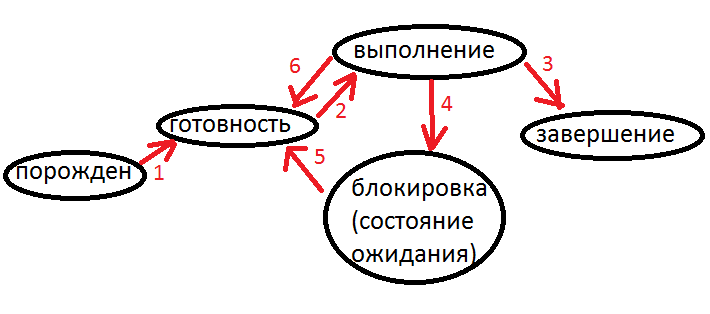
\includegraphics[width=\textwidth]{pic/2.png}
  \caption{Самая общая диаграмма состояний процесса}
  \label{pic:diag_proc}
\end{figure}

Процесс в начале идентифицируется. В системе есть одна на систему таблицы процессов. Любая системная таблица – массив структур. Процесс в системе описывается структурой proc. Каждому запущенному процессу выделяется структура (дескриптор) процесса (строка в таблице процессов). Номер строки – это id процесса, целое число. 

На \ref{pic:diag_proc} ребро 1 – выделяется первый необходимый ресурс – объем ОЗУ, в соответствии с концепцией хранимой программы и переходит в состояние готовности.

В состоянии готовности находится большое количество процессов. Они составляют очередь. В очереди процессы располагаются с приоритетами. Процессорное время получает самый приоритетный. Если в очередь поступил наиболее приоритетный процесс, чем тот, какой выполняется сейчас, то он вытесняется. Это реализуется в системах пакетной обработки и реального времени.

В разделении времени ???

В системах квантования при истечении кванта, процесс возвращается в очередь. При вытеснении происходит переключение контекста. Если процесс вытеснен или исчерпан квант, то необходимо сохранить информацию, которая поможет продолжению выполнения. 
\textbf{Полный контекст} – информация о выделенных процессу ресурсов + аппаратный контекст.
???

\paragraph{Уровни наблюдения}: 
\begin{enumerate}
	\item последовательное выполнение.
	\item квазипараллельное выполнение. (с точки зрения пользователя – параллельно)
	\item реальная параллельность.
\end{enumerate}

\paragraph{Планирование и диспетчеризация}: 
\begin{enumerate}
	\item безприоритетное
	\item приоритетное
\end{enumerate}

\paragraph{Приоритеты}: 
\begin{enumerate}
	\item абсолютные и относительные;
	\item статические и динамические.
\end{enumerate}

\paragraph{Планирование}: 
\begin{enumerate}
	\item с переключением и без;
	\item с выталкиванием и без.
\end{enumerate}
